% pdflatex linear_parameters.tex
% convert -density 600 linear_parameters.pdf linear_parameters.png

\documentclass[tikz,convert={outfile=\jobname.png},margin=2mm]{standalone}
%\usetikzlibrary{...}% tikz package already loaded by 'tikz' option

\usepackage{amssymb,amsmath}
\usepackage{bm}
\DeclareMathSymbol{\shortminus}{\mathbin}{AMSa}{"39}
\newcommand{\half}{\text{\textonehalf}}
\renewcommand{\t}{\mathsf{T}}
\newcommand{\T}{\mkern-3mu}

\usetikzlibrary{angles,quotes}
\begin{document}
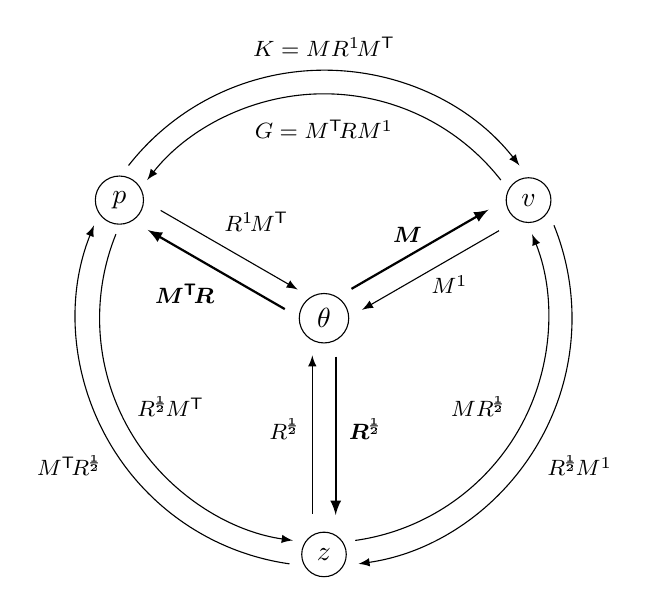
\begin{tikzpicture}

    \def \n {3}
    \def \radius {3cm}
    \def \margin {8} % margin in angles, depends on the radius


    \node[draw, circle] at ({30 + 360/3 * 0}:\radius) {$v$};
    \node[draw, circle] at ({30 + 360/3 * 1}:\radius) {$p$};
    \node[draw, circle] at ({30 + 360/3 * 2}:\radius) {$z$};
    \node[draw, circle] at (0, 0) {$\theta$};

    % p <-> v
    \node at ({90 + 360/3 * 0}:1.15*\radius) {\footnotesize $K = M R^{\shortminus1}\T M^\t$};
    \node at ({90 + 360/3 * 0}:0.80*\radius) {\footnotesize $G = M^{\shortminus\t} \T R M^{\shortminus1}$};

    % p <-> z
    \node at ({90 + 360/3 * 1}:1.25*\radius) {\footnotesize $M^{\shortminus\t}\T R^{\half}$};
    \node at ({90 + 360/3 * 1}:0.75*\radius) {\footnotesize $R^{\shortminus \half} M^\t$};

    % z <-> v
    \node at ({90 + 360/3 * 2}:1.25*\radius) {\footnotesize $R^{\half} M^{\shortminus 1} $};
    \node at ({90 + 360/3 * 2}:0.75*\radius) {\footnotesize $M R^{\shortminus \half}$};


    % theta <-> v
    \node at ({30 + 15 + 360/3 * 0}:.5*\radius) {\footnotesize $\bm{M}$};
    \node at ({30 - 15 + 360/3 * 0}:.55*\radius) {\footnotesize $M^{\shortminus 1}$};

    % theta <-> p
    \node at ({30 + 20 + 360/3 * 1}:.6*\radius) {\footnotesize $\bm{M^{\shortminus\t}\T R}$};
    \node at ({30 - 25 + 360/3 * 1}:.5*\radius) {\footnotesize $R^{\shortminus 1}\T M^{\t}$};

    % theta <-> z
    \node at ({30 + 20 + 360/3 * 2}:.5*\radius) {\footnotesize $\bm{R^{\half}}$};
    \node at ({30 - 20 + 360/3 * 2}:.5*\radius) {\footnotesize $R^{\shortminus \half}$};




    \foreach \s in {1,...,\n}
    {
      \draw[->, >=latex] ({30 + 360/\n * (\s - 1)+\margin}:0.95*\radius)
        arc ({30 + 360/\n * (\s - 1)+\margin}:{30 + 360/\n * (\s)-\margin}:0.95*\radius);
      \draw[<-, >=latex] ({30 + 360/\n * (\s - 1)+\margin}:1.05*\radius)
        arc ({30 + 360/\n * (\s - 1)+\margin}:{30 + 360/\n * (\s)-\margin}:1.05*\radius);

      \draw[->, >=latex, thick, shift={({90 + 30 + 360/\n * (\s - 1)+\margin}:.15)}] ({30 + 360/\n * (\s - 1)}:0.17*\radius)
        -- ({30 + 360/\n * (\s - 1)}:0.84*\radius);
      \draw[<-, >=latex, shift={({-90 + 30 + 360/\n * (\s - 1)+\margin}:.15)}] ({30 + 360/\n * (\s - 1)}:0.15*\radius)
        -- ({30 + 360/\n * (\s - 1)}:0.82*\radius);

    }
    \end{tikzpicture}
\end{document}
